% ============================================================
%  Information Theory --- Module 1 --- ALL DIAGRAMS (merged)
%  Compile with pdfLaTeX.  Each diagram starts on its own page.
%  Auto-merged from Information_Theory_Module1_Solutions.md
% ============================================================
\documentclass[11pt]{article}
\usepackage[a4paper,margin=1.5cm]{geometry}
\usepackage{amsmath}
\usepackage{tikz}
\usetikzlibrary{automata,positioning,arrows.meta,trees,calc}
\usepackage{forest}
\usepackage{pgfplots}
\pgfplotsset{compat=1.18}
\setlength{\parindent}{0pt}
\title{\textbf{Information Theory --- Module 1}\\[2pt] All Diagrams (TikZ / forest / pgfplots)}
\author{}
\date{}
\begin{document}
\maketitle

% ---------- Q7 : diagram 1 ----------
\clearpage
\section*{Q7 --- diagram 1}
\begin{center}
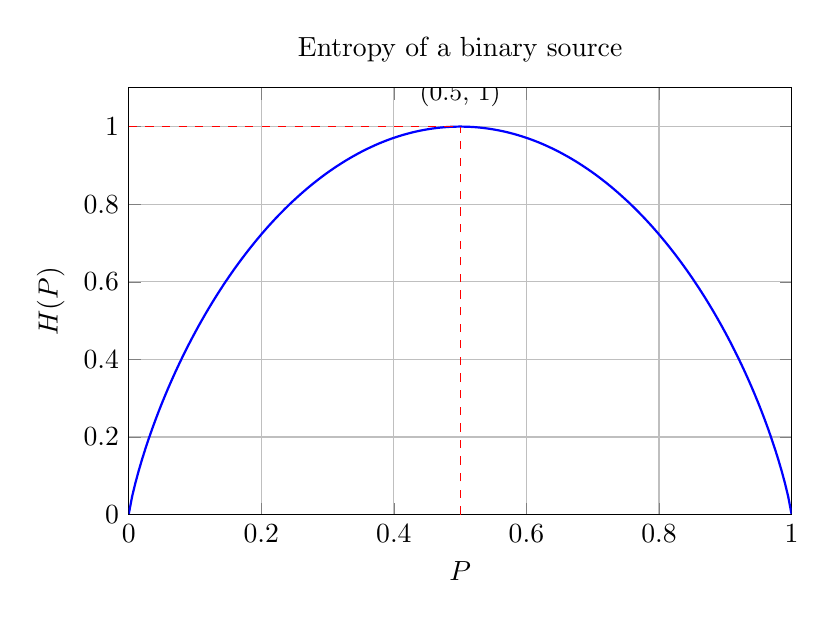
\begin{tikzpicture}
\begin{axis}[
    xlabel=$P$, ylabel=$H(P)$,
    xmin=0, xmax=1, ymin=0, ymax=1.1,
    samples=200, domain=0.0001:0.9999,
    grid=both, width=10cm, height=7cm,
    title={Entropy of a binary source}]
\addplot[blue,thick]{-x*ln(x)/ln(2)-(1-x)*ln(1-x)/ln(2)};
\addplot[dashed,red] coordinates {(0.5,0)(0.5,1)};
\addplot[dashed,red] coordinates {(0,1)(0.5,1)};
\node[label={[font=\small]above:$(0.5,\,1)$}] at (axis cs:0.5,1){};
\end{axis}
\end{tikzpicture}
\end{center}

% ---------- Q11 : diagram 2 ----------
\clearpage
\section*{Q11 --- diagram 2}
\begin{center}
\begin{forest}
for tree={grow'=east, parent anchor=east, child anchor=west,
          edge={-stealth}, l sep=16mm, s sep=2mm, font=\footnotesize}
[{Start}
  [{$1$ $\tfrac13$}, edge label={node[midway,above,font=\tiny]{$\tfrac13$}}
    [{$11=\tfrac16$},   edge label={node[midway,above,font=\tiny]{$\tfrac12$}}]
    [{$12=\tfrac1{12}$},edge label={node[midway,above,font=\tiny]{$\tfrac14$}}]
    [{$13=\tfrac1{12}$},edge label={node[midway,below,font=\tiny]{$\tfrac14$}}]
  ]
  [{$2$ $\tfrac13$}, edge label={node[midway,above,font=\tiny]{$\tfrac13$}}
    [{$21=\tfrac1{12}$},edge label={node[midway,above,font=\tiny]{$\tfrac14$}}]
    [{$22=\tfrac16$},   edge label={node[midway,above,font=\tiny]{$\tfrac12$}}]
    [{$23=\tfrac1{12}$},edge label={node[midway,below,font=\tiny]{$\tfrac14$}}]
  ]
  [{$3$ $\tfrac13$}, edge label={node[midway,below,font=\tiny]{$\tfrac13$}}
    [{$31=\tfrac1{12}$},edge label={node[midway,above,font=\tiny]{$\tfrac14$}}]
    [{$32=\tfrac1{12}$},edge label={node[midway,above,font=\tiny]{$\tfrac14$}}]
    [{$33=\tfrac16$},   edge label={node[midway,below,font=\tiny]{$\tfrac12$}}]
  ]
]
\end{forest}
\end{center}

% ---------- Q11 : diagram 3 ----------
\clearpage
\section*{Q11 --- diagram 3}
\begin{center}
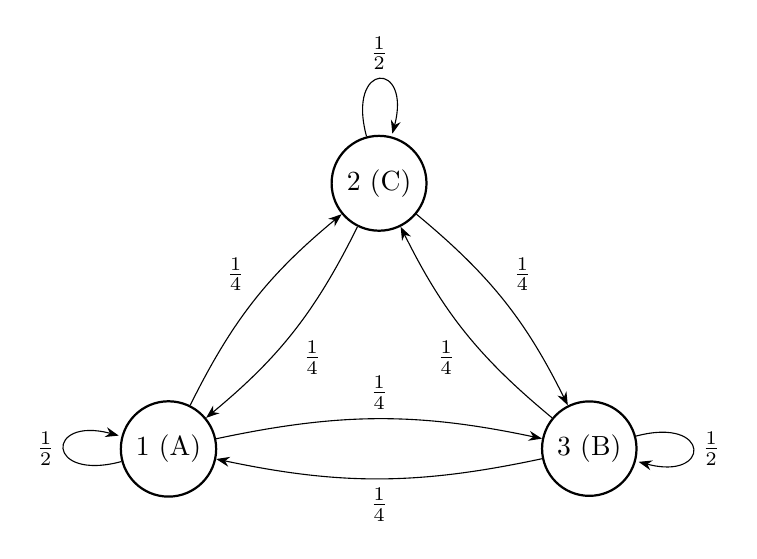
\begin{tikzpicture}[->,>=Stealth,auto,node distance=3.5cm,
   every state/.style={thick,minimum size=1cm}]
  \node[state] (S2) {2 (C)};
  \node[state] (S1) [below left=2.5cm and 1.8cm of S2] {1 (A)};
  \node[state] (S3) [below right=2.5cm and 1.8cm of S2] {3 (B)};
  \path
    (S1) edge[loop left]  node{$\tfrac12$} (S1)
    (S2) edge[loop above] node{$\tfrac12$} (S2)
    (S3) edge[loop right] node{$\tfrac12$} (S3)
    (S1) edge[bend left=12]  node{$\tfrac14$} (S2)
    (S2) edge[bend left=12]  node{$\tfrac14$} (S1)
    (S2) edge[bend left=12]  node{$\tfrac14$} (S3)
    (S3) edge[bend left=12]  node{$\tfrac14$} (S2)
    (S1) edge[bend left=12]  node{$\tfrac14$} (S3)
    (S3) edge[bend left=12]  node{$\tfrac14$} (S1);
\end{tikzpicture}
\end{center}

% ---------- Q12 : diagram 4 ----------
\clearpage
\section*{Q12 --- diagram 4}
\begin{center}
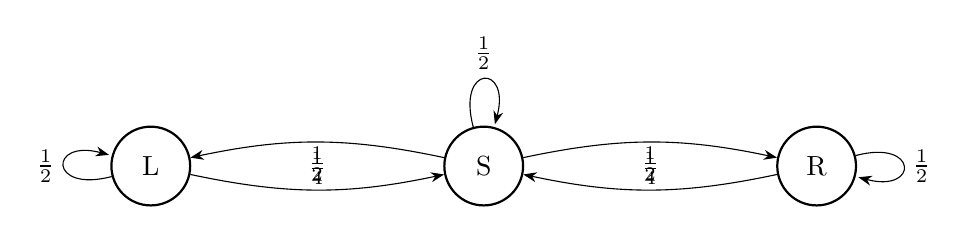
\begin{tikzpicture}[->,>=Stealth,auto,node distance=3.2cm,
   every state/.style={thick,minimum size=1cm}]
  \node[state] (S) {S};
  \node[state] (L) [left=of S] {L};
  \node[state] (R) [right=of S] {R};
  \path
   (S) edge[loop above] node{$\tfrac12$} (S)
   (L) edge[loop left]  node{$\tfrac12$} (L)
   (R) edge[loop right] node{$\tfrac12$} (R)
   (S) edge[bend right=12] node[below]{$\tfrac14$} (L)
   (L) edge[bend right=12] node[above]{$\tfrac12$} (S)
   (S) edge[bend left=12]  node[below]{$\tfrac14$} (R)
   (R) edge[bend left=12]  node[above]{$\tfrac12$} (S);
\end{tikzpicture}
\end{center}

% ---------- Q13 : diagram 5 ----------
\clearpage
\section*{Q13 --- diagram 5}
\begin{center}
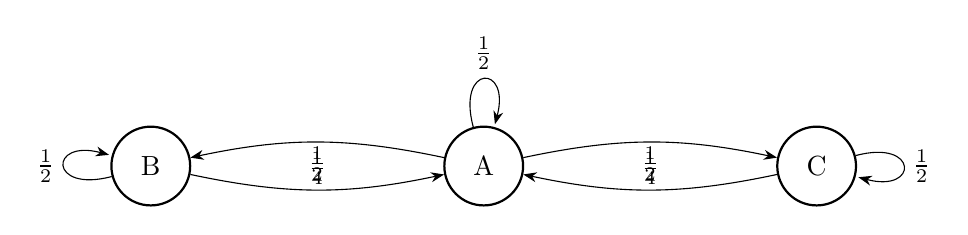
\begin{tikzpicture}[->,>=Stealth,auto,node distance=3.2cm,
   every state/.style={thick,minimum size=1cm}]
  \node[state] (A) {A};
  \node[state] (B) [left=of A] {B};
  \node[state] (C) [right=of A] {C};
  \path
   (A) edge[loop above] node{$\tfrac12$} (A)
   (B) edge[loop left]  node{$\tfrac12$} (B)
   (C) edge[loop right] node{$\tfrac12$} (C)
   (A) edge[bend right=12] node[below]{$\tfrac14$} (B)
   (B) edge[bend right=12] node[above]{$\tfrac12$} (A)
   (A) edge[bend left=12]  node[below]{$\tfrac14$} (C)
   (C) edge[bend left=12]  node[above]{$\tfrac12$} (A);
\end{tikzpicture}
\end{center}

% ---------- Q14 : diagram 6 ----------
\clearpage
\section*{Q14 --- diagram 6}
\begin{center}
\begin{forest}
for tree={grow'=east, parent anchor=east, child anchor=west,
          edge={-stealth}, l sep=20mm, s sep=1.5mm, font=\footnotesize}
[{Start}
  [{$1$ $\tfrac{3}{7}$}, edge label={node[midway,above,font=\tiny]{$\tfrac37$}}
    [{$X{:}1$ $\tfrac{2}{7}$}, edge label={node[midway,above,font=\tiny]{$X\,\tfrac23$}}
      [{$X{:}1$ $\tfrac{4}{21}$}, edge label={node[midway,above,font=\tiny]{$X\,\tfrac23$}}
        [{$XXX=\tfrac{8}{63}$},  edge label={node[midway,above,font=\tiny]{$X\,\tfrac23$}}]
        [{$XXZ=\tfrac{4}{63}$},  edge label={node[midway,below,font=\tiny]{$Z\,\tfrac13$}}]]
      [{$Z{:}2$ $\tfrac{2}{21}$}, edge label={node[midway,below,font=\tiny]{$Z\,\tfrac13$}}
        [{$XZZ=\tfrac{1}{42}$},  edge label={node[midway,above,font=\tiny]{$Z\,\tfrac14$}}]
        [{$XZY=\tfrac{1}{14}$},  edge label={node[midway,below,font=\tiny]{$Y\,\tfrac34$}}]]]
    [{$Z{:}2$ $\tfrac{1}{7}$}, edge label={node[midway,below,font=\tiny]{$Z\,\tfrac13$}}
      [{$Z{:}1$ $\tfrac{1}{28}$}, edge label={node[midway,above,font=\tiny]{$Z\,\tfrac14$}}
        [{$ZZX=\tfrac{1}{42}$},  edge label={node[midway,above,font=\tiny]{$X\,\tfrac23$}}]
        [{$ZZZ=\tfrac{1}{84}$},  edge label={node[midway,below,font=\tiny]{$Z\,\tfrac13$}}]]
      [{$Y{:}2$ $\tfrac{3}{28}$}, edge label={node[midway,below,font=\tiny]{$Y\,\tfrac34$}}
        [{$ZYZ=\tfrac{3}{112}$}, edge label={node[midway,above,font=\tiny]{$Z\,\tfrac14$}}]
        [{$ZYY=\tfrac{9}{112}$}, edge label={node[midway,below,font=\tiny]{$Y\,\tfrac34$}}]]]]
  [{$2$ $\tfrac{4}{7}$}, edge label={node[midway,below,font=\tiny]{$\tfrac47$}}
    [{$Z{:}1$ $\tfrac{1}{7}$}, edge label={node[midway,above,font=\tiny]{$Z\,\tfrac14$}}
      [{$X{:}1$ $\tfrac{2}{21}$}, edge label={node[midway,above,font=\tiny]{$X\,\tfrac23$}}
        [{$ZXX=\tfrac{4}{63}$},  edge label={node[midway,above,font=\tiny]{$X\,\tfrac23$}}]
        [{$ZXZ=\tfrac{2}{63}$},  edge label={node[midway,below,font=\tiny]{$Z\,\tfrac13$}}]]
      [{$Z{:}2$ $\tfrac{1}{21}$}, edge label={node[midway,below,font=\tiny]{$Z\,\tfrac13$}}
        [{$ZZZ=\tfrac{1}{84}$},  edge label={node[midway,above,font=\tiny]{$Z\,\tfrac14$}}]
        [{$ZZY=\tfrac{1}{28}$},  edge label={node[midway,below,font=\tiny]{$Y\,\tfrac34$}}]]]
    [{$Y{:}2$ $\tfrac{3}{7}$}, edge label={node[midway,below,font=\tiny]{$Y\,\tfrac34$}}
      [{$Z{:}1$ $\tfrac{3}{28}$}, edge label={node[midway,above,font=\tiny]{$Z\,\tfrac14$}}
        [{$YZX=\tfrac{1}{14}$},  edge label={node[midway,above,font=\tiny]{$X\,\tfrac23$}}]
        [{$YZZ=\tfrac{1}{28}$},  edge label={node[midway,below,font=\tiny]{$Z\,\tfrac13$}}]]
      [{$Y{:}2$ $\tfrac{9}{28}$}, edge label={node[midway,below,font=\tiny]{$Y\,\tfrac34$}}
        [{$YYZ=\tfrac{9}{112}$}, edge label={node[midway,above,font=\tiny]{$Z\,\tfrac14$}}]
        [{$YYY=\tfrac{27}{112}$},edge label={node[midway,below,font=\tiny]{$Y\,\tfrac34$}}]]]]
]
\end{forest}
\end{center}

% ---------- Q14 : diagram 7 ----------
\clearpage
\section*{Q14 --- diagram 7}
\begin{center}
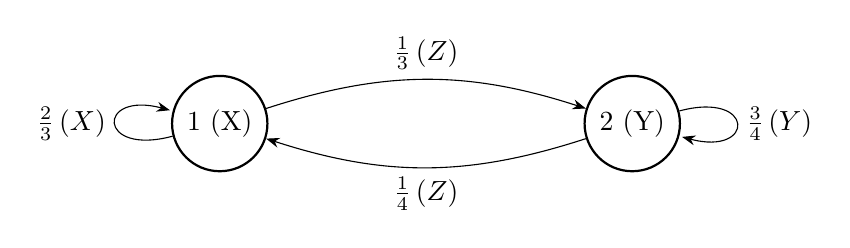
\begin{tikzpicture}[->,>=Stealth,auto,node distance=4cm,
   every state/.style={thick,minimum size=1.1cm}]
  \node[state] (s1) {1 (X)};
  \node[state] (s2) [right=of s1] {2 (Y)};
  \path
   (s1) edge[loop left]  node{$\tfrac23\,(X)$} (s1)
   (s2) edge[loop right] node{$\tfrac34\,(Y)$} (s2)
   (s1) edge[bend left=18] node[above]{$\tfrac13\,(Z)$} (s2)
   (s2) edge[bend left=18] node[below]{$\tfrac14\,(Z)$} (s1);
\end{tikzpicture}
\end{center}

% ---------- Q15 : diagram 8 ----------
\clearpage
\section*{Q15 --- diagram 8}
\begin{center}
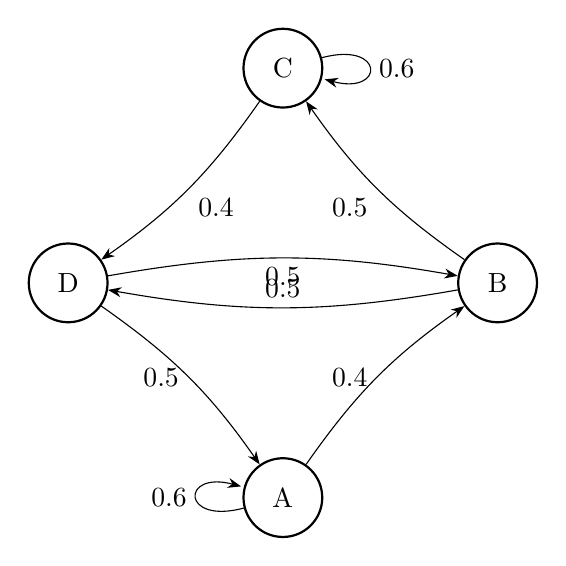
\begin{tikzpicture}[->,>=Stealth,auto,node distance=2.8cm,
   every state/.style={thick,minimum size=1cm}]
  \node[state] (C) {C};
  \node[state] (D) [below left=2cm and 2cm of C] {D};
  \node[state] (B) [below right=2cm and 2cm of C] {B};
  \node[state] (A) [below right=2cm and 2cm of D] {A};
  \path
   (A) edge[loop left]  node{$0.6$} (A)
   (C) edge[loop right] node{$0.6$} (C)
   (A) edge[bend left=10] node[left]{$0.4$} (B)
   (B) edge[bend left=10] node{$0.5$} (C)
   (C) edge[bend left=10] node{$0.4$} (D)
   (D) edge[bend left=10] node[left]{$0.5$} (A)
   (B) edge[bend left=10] node[above]{$0.5$} (D)
   (D) edge[bend left=10] node[below]{$0.5$} (B);
\end{tikzpicture}
\end{center}

% ---------- Q16 : diagram 9 ----------
\clearpage
\section*{Q16 --- diagram 9}
\begin{center}
\begin{forest}
for tree={grow'=east, parent anchor=east, child anchor=west,
          edge={-stealth}, l sep=16mm, s sep=2mm, font=\footnotesize}
[{Start}
  [{$A$ $\tfrac13$}, edge label={node[midway,above,font=\tiny]{$\tfrac13$}}
    [{$AA=0.200$}, edge label={node[midway,above,font=\tiny]{$0.6$}}]
    [{$AB=0.067$}, edge label={node[midway,above,font=\tiny]{$0.2$}}]
    [{$AC=0.067$}, edge label={node[midway,below,font=\tiny]{$0.2$}}]]
  [{$B$ $\tfrac13$}, edge label={node[midway,above,font=\tiny]{$\tfrac13$}}
    [{$BA=0.100$}, edge label={node[midway,above,font=\tiny]{$0.3$}}]
    [{$BB=0.167$}, edge label={node[midway,above,font=\tiny]{$0.5$}}]
    [{$BC=0.067$}, edge label={node[midway,below,font=\tiny]{$0.2$}}]]
  [{$C$ $\tfrac13$}, edge label={node[midway,below,font=\tiny]{$\tfrac13$}}
    [{$CA=0.100$}, edge label={node[midway,above,font=\tiny]{$0.3$}}]
    [{$CB=0.100$}, edge label={node[midway,above,font=\tiny]{$0.3$}}]
    [{$CC=0.133$}, edge label={node[midway,below,font=\tiny]{$0.4$}}]]
]
\end{forest}
\end{center}

% ---------- Q16 : diagram 10 ----------
\clearpage
\section*{Q16 --- diagram 10}
\begin{center}
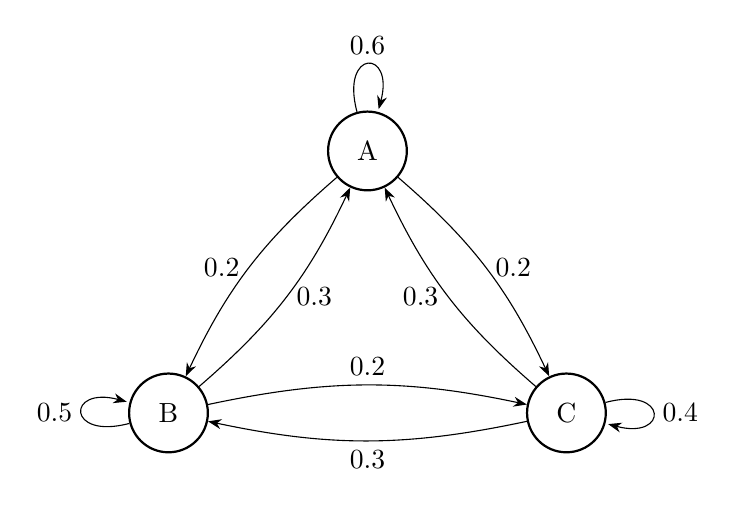
\begin{tikzpicture}[->,>=Stealth,auto,node distance=3.6cm,
   every state/.style={thick,minimum size=1cm}]
  \node[state] (A) {A};
  \node[state] (B) [below left=2.6cm and 1.8cm of A] {B};
  \node[state] (C) [below right=2.6cm and 1.8cm of A] {C};
  \path
   (A) edge[loop above] node{$0.6$} (A)
   (B) edge[loop left]  node{$0.5$} (B)
   (C) edge[loop right] node{$0.4$} (C)
   (A) edge[bend right=12] node[left]{$0.2$} (B)
   (B) edge[bend right=12] node[right]{$0.3$} (A)
   (A) edge[bend left=12]  node[right]{$0.2$} (C)
   (C) edge[bend left=12]  node[left]{$0.3$} (A)
   (B) edge[bend left=12]  node[above]{$0.2$} (C)
   (C) edge[bend left=12]  node[below]{$0.3$} (B);
\end{tikzpicture}
\end{center}

% ---------- Q17 : diagram 11 ----------
\clearpage
\section*{Q17 --- diagram 11}
\begin{center}
\begin{forest}
for tree={grow'=east, parent anchor=east, child anchor=west,
          edge={-stealth}, l sep=20mm, s sep=1.5mm, font=\footnotesize}
[{Start}
  [{$1$ $\tfrac12$}, edge label={node[midway,above,font=\tiny]{$\tfrac12$}}
    [{$A{:}1$ $\tfrac38$}, edge label={node[midway,above,font=\tiny]{$A\,\tfrac34$}}
      [{$A{:}1$ $\tfrac{9}{32}$}, edge label={node[midway,above,font=\tiny]{$A\,\tfrac34$}}
        [{$AAA=\tfrac{27}{128}$}, edge label={node[midway,above,font=\tiny]{$A\,\tfrac34$}}]
        [{$AAC=\tfrac{9}{128}$},  edge label={node[midway,below,font=\tiny]{$C\,\tfrac14$}}]]
      [{$C{:}2$ $\tfrac{3}{32}$}, edge label={node[midway,below,font=\tiny]{$C\,\tfrac14$}}
        [{$ACC=\tfrac{3}{128}$},  edge label={node[midway,above,font=\tiny]{$C\,\tfrac14$}}]
        [{$ACB=\tfrac{9}{128}$},  edge label={node[midway,below,font=\tiny]{$B\,\tfrac34$}}]]]
    [{$C{:}2$ $\tfrac18$}, edge label={node[midway,below,font=\tiny]{$C\,\tfrac14$}}
      [{$C{:}1$ $\tfrac{1}{32}$}, edge label={node[midway,above,font=\tiny]{$C\,\tfrac14$}}
        [{$CCA=\tfrac{3}{128}$},  edge label={node[midway,above,font=\tiny]{$A\,\tfrac34$}}]
        [{$CCC=\tfrac{1}{128}$},  edge label={node[midway,below,font=\tiny]{$C\,\tfrac14$}}]]
      [{$B{:}2$ $\tfrac{3}{32}$}, edge label={node[midway,below,font=\tiny]{$B\,\tfrac34$}}
        [{$CBC=\tfrac{3}{128}$},  edge label={node[midway,above,font=\tiny]{$C\,\tfrac14$}}]
        [{$CBB=\tfrac{9}{128}$},  edge label={node[midway,below,font=\tiny]{$B\,\tfrac34$}}]]]]
  [{$2$ $\tfrac12$}, edge label={node[midway,below,font=\tiny]{$\tfrac12$}}
    [{$C{:}1$ $\tfrac18$}, edge label={node[midway,above,font=\tiny]{$C\,\tfrac14$}}
      [{$A{:}1$ $\tfrac{3}{32}$}, edge label={node[midway,above,font=\tiny]{$A\,\tfrac34$}}
        [{$CAA=\tfrac{9}{128}$},  edge label={node[midway,above,font=\tiny]{$A\,\tfrac34$}}]
        [{$CAC=\tfrac{3}{128}$},  edge label={node[midway,below,font=\tiny]{$C\,\tfrac14$}}]]
      [{$C{:}2$ $\tfrac{1}{32}$}, edge label={node[midway,below,font=\tiny]{$C\,\tfrac14$}}
        [{$CCC=\tfrac{1}{128}$},  edge label={node[midway,above,font=\tiny]{$C\,\tfrac14$}}]
        [{$CCB=\tfrac{3}{128}$},  edge label={node[midway,below,font=\tiny]{$B\,\tfrac34$}}]]]
    [{$B{:}2$ $\tfrac38$}, edge label={node[midway,below,font=\tiny]{$B\,\tfrac34$}}
      [{$C{:}1$ $\tfrac{3}{32}$}, edge label={node[midway,above,font=\tiny]{$C\,\tfrac14$}}
        [{$BCA=\tfrac{9}{128}$},  edge label={node[midway,above,font=\tiny]{$A\,\tfrac34$}}]
        [{$BCC=\tfrac{3}{128}$},  edge label={node[midway,below,font=\tiny]{$C\,\tfrac14$}}]]
      [{$B{:}2$ $\tfrac{9}{32}$}, edge label={node[midway,below,font=\tiny]{$B\,\tfrac34$}}
        [{$BBC=\tfrac{9}{128}$},  edge label={node[midway,above,font=\tiny]{$C\,\tfrac14$}}]
        [{$BBB=\tfrac{27}{128}$}, edge label={node[midway,below,font=\tiny]{$B\,\tfrac34$}}]]]]
]
\end{forest}
\end{center}

% ---------- Q17 : diagram 12 ----------
\clearpage
\section*{Q17 --- diagram 12}
\begin{center}
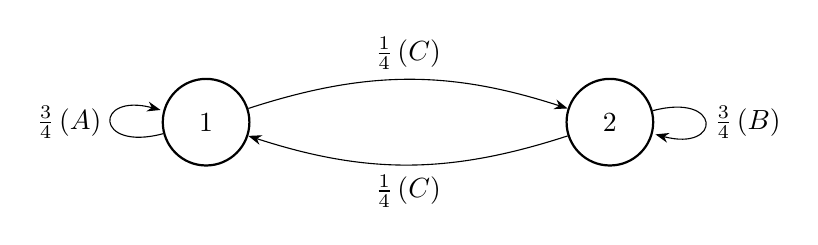
\begin{tikzpicture}[->,>=Stealth,auto,node distance=4cm,
   every state/.style={thick,minimum size=1.1cm}]
  \node[state] (s1) {1};
  \node[state] (s2) [right=of s1] {2};
  \path
   (s1) edge[loop left]  node{$\tfrac34\,(A)$} (s1)
   (s2) edge[loop right] node{$\tfrac34\,(B)$} (s2)
   (s1) edge[bend left=18] node[above]{$\tfrac14\,(C)$} (s2)
   (s2) edge[bend left=18] node[below]{$\tfrac14\,(C)$} (s1);
\end{tikzpicture}
\end{center}

% ---------- Q18 : diagram 13 ----------
\clearpage
\section*{Q18 --- diagram 13}
\begin{center}
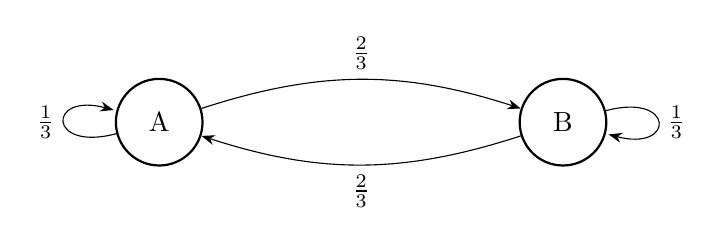
\begin{tikzpicture}[->,>=Stealth,auto,node distance=4cm,
   every state/.style={thick,minimum size=1.1cm}]
  \node[state] (A) {A};
  \node[state] (B) [right=of A] {B};
  \path
   (A) edge[loop left]  node{$\tfrac13$} (A)
   (B) edge[loop right] node{$\tfrac13$} (B)
   (A) edge[bend left=18] node[above]{$\tfrac23$} (B)
   (B) edge[bend left=18] node[below]{$\tfrac23$} (A);
\end{tikzpicture}
\end{center}

% ---------- Q19 : diagram 14 ----------
\clearpage
\section*{Q19 --- diagram 14}
\begin{center}
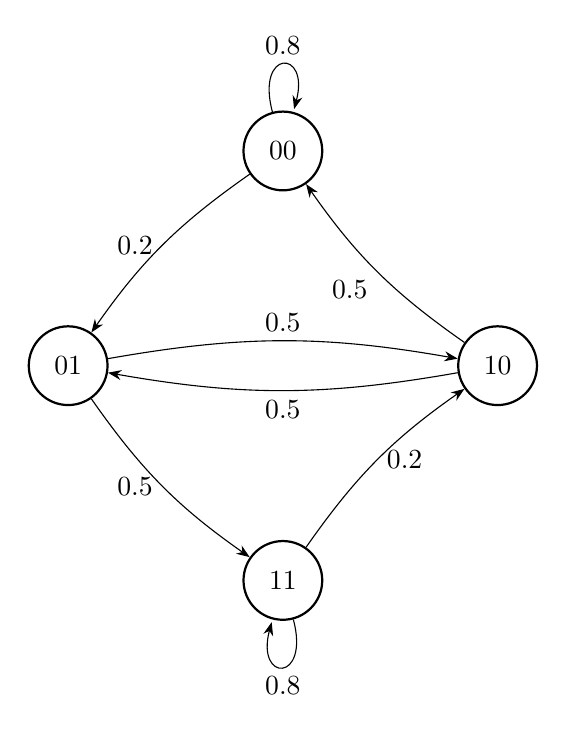
\begin{tikzpicture}[->,>=Stealth,auto,node distance=2.8cm,
   every state/.style={thick,minimum size=1cm}]
  \node[state] (a) {00};
  \node[state] (b) [below left=2cm and 2cm of a] {01};
  \node[state] (c) [below right=2cm and 2cm of a] {10};
  \node[state] (d) [below right=2cm and 2cm of b] {11};
  \path
   (a) edge[loop above] node{$0.8$} (a)
   (d) edge[loop below] node{$0.8$} (d)
   (a) edge[bend right=10] node[left]{$0.2$} (b)
   (b) edge[bend left=10]  node{$0.5$} (c)
   (c) edge[bend left=10]  node{$0.5$} (b)
   (c) edge[bend left=10]  node{$0.5$} (a)
   (b) edge[bend right=10] node[left]{$0.5$} (d)
   (d) edge[bend left=10]  node[right]{$0.2$} (c);
\end{tikzpicture}
\end{center}

% ---------- Q20 : diagram 15 ----------
\clearpage
\section*{Q20 --- diagram 15}
\begin{center}
\begin{forest}
for tree={grow'=east, parent anchor=east, child anchor=west,
          edge={-stealth}, l sep=20mm, s sep=1.5mm, font=\footnotesize}
[{Start}
  [{$1$ $0.783$}, edge label={node[midway,above,font=\tiny]{$0.783$}}
    [{$X{:}1$ $0.652$}, edge label={node[midway,above,font=\tiny]{$X\,\tfrac56$}}
      [{$X{:}1$ $0.5435$}, edge label={node[midway,above,font=\tiny]{$X\,\tfrac56$}}
        [{$XXX=0.4529$}, edge label={node[midway,above,font=\tiny]{$X\,\tfrac56$}}]
        [{$XXZ=0.0906$}, edge label={node[midway,below,font=\tiny]{$Z\,\tfrac16$}}]]
      [{$Z{:}2$ $0.1087$}, edge label={node[midway,below,font=\tiny]{$Z\,\tfrac16$}}
        [{$XZZ=0.0652$}, edge label={node[midway,above,font=\tiny]{$Z\,\tfrac35$}}]
        [{$XZY=0.0435$}, edge label={node[midway,below,font=\tiny]{$Y\,\tfrac25$}}]]]
    [{$Z{:}2$ $0.1304$}, edge label={node[midway,below,font=\tiny]{$Z\,\tfrac16$}}
      [{$Z{:}1$ $0.0783$}, edge label={node[midway,above,font=\tiny]{$Z\,\tfrac35$}}
        [{$ZZX=0.0652$}, edge label={node[midway,above,font=\tiny]{$X\,\tfrac56$}}]
        [{$ZZZ=0.0130$}, edge label={node[midway,below,font=\tiny]{$Z\,\tfrac16$}}]]
      [{$Y{:}2$ $0.0522$}, edge label={node[midway,below,font=\tiny]{$Y\,\tfrac25$}}
        [{$ZYZ=0.0313$}, edge label={node[midway,above,font=\tiny]{$Z\,\tfrac35$}}]
        [{$ZYY=0.0209$}, edge label={node[midway,below,font=\tiny]{$Y\,\tfrac25$}}]]]]
  [{$2$ $0.217$}, edge label={node[midway,below,font=\tiny]{$0.217$}}
    [{$Z{:}1$ $0.1304$}, edge label={node[midway,above,font=\tiny]{$Z\,\tfrac35$}}
      [{$X{:}1$ $0.1087$}, edge label={node[midway,above,font=\tiny]{$X\,\tfrac56$}}
        [{$ZXX=0.0906$}, edge label={node[midway,above,font=\tiny]{$X\,\tfrac56$}}]
        [{$ZXZ=0.0181$}, edge label={node[midway,below,font=\tiny]{$Z\,\tfrac16$}}]]
      [{$Z{:}2$ $0.0217$}, edge label={node[midway,below,font=\tiny]{$Z\,\tfrac16$}}
        [{$ZZZ=0.0130$}, edge label={node[midway,above,font=\tiny]{$Z\,\tfrac35$}}]
        [{$ZZY=0.0087$}, edge label={node[midway,below,font=\tiny]{$Y\,\tfrac25$}}]]]
    [{$Y{:}2$ $0.0870$}, edge label={node[midway,below,font=\tiny]{$Y\,\tfrac25$}}
      [{$Z{:}1$ $0.0522$}, edge label={node[midway,above,font=\tiny]{$Z\,\tfrac35$}}
        [{$YZX=0.0435$}, edge label={node[midway,above,font=\tiny]{$X\,\tfrac56$}}]
        [{$YZZ=0.0087$}, edge label={node[midway,below,font=\tiny]{$Z\,\tfrac16$}}]]
      [{$Y{:}2$ $0.0348$}, edge label={node[midway,below,font=\tiny]{$Y\,\tfrac25$}}
        [{$YYZ=0.0209$}, edge label={node[midway,above,font=\tiny]{$Z\,\tfrac35$}}]
        [{$YYY=0.0139$}, edge label={node[midway,below,font=\tiny]{$Y\,\tfrac25$}}]]]]
]
\end{forest}
\end{center}

% ---------- Q20 : diagram 16 ----------
\clearpage
\section*{Q20 --- diagram 16}
\begin{center}
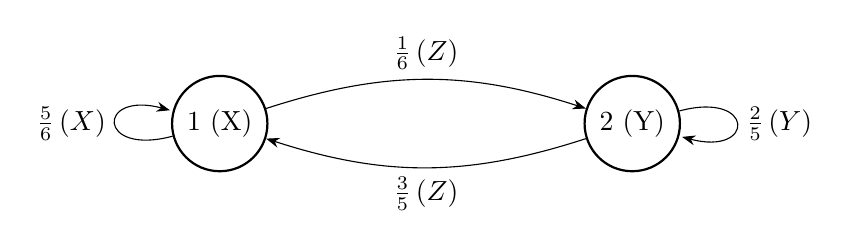
\begin{tikzpicture}[->,>=Stealth,auto,node distance=4cm,
   every state/.style={thick,minimum size=1.1cm}]
  \node[state] (s1) {1 (X)};
  \node[state] (s2) [right=of s1] {2 (Y)};
  \path
   (s1) edge[loop left]  node{$\tfrac56\,(X)$} (s1)
   (s2) edge[loop right] node{$\tfrac25\,(Y)$} (s2)
   (s1) edge[bend left=18] node[above]{$\tfrac16\,(Z)$} (s2)
   (s2) edge[bend left=18] node[below]{$\tfrac35\,(Z)$} (s1);
\end{tikzpicture}
\end{center}

\end{document}
